\section{Аналого-цифровые преобразователи}

%В NA64 для оцифровки сигнала с \acrshort{pmt} счётчиков, вето-детекторов и
%калориметров применяются аналого-цифровые преобразователи MSADC \cite{MSADC-Mann1, %MSADC-Mann2} (\emph{англ} Mezzanine sampling analog to digital converted).
Для оцифровки сигналов формируемых \acrshort{pmt} (пучковых счётчиков,
вето-детекторов и калориметров) в NA64 применяются
аналого-цифровые преобразователи MSADC \cite{MSADC-Mann1, MSADC-Mann2}
(англ. \emph{Mezzanine Sampling Analog-to-Digital Converter}).
MSADC представляет собой устройство на основе микросхемы
ADS527x~\cite{ADS527x}, выполненное в виде мезонинной карты расширения
в стандарте <<Advanced Telecom Computing Architecture>> (ATCA).
Конструктивно, предусмотрен монтаж устройства как в
корзину (крейт) системы сбора данных, так и в непосредственной близи
детекторной сборки для уменьшения длин аналоговых линий и уменьшения помех.
MSADC в установке NA64 применяются как для непосредственного считывания
сигналов \acrshort{pmt}, так и опосредованно, для оцифровки сигналов
от микропаттерных детекторов предварительно подаваемых на вход
аналогового демультиплексора.

В рамках первого сценария каждый аналоговый канал считывается двумя сэмплирующими
АЦП, работающими на частоте $40\text{МГц}$. Каналы тактируются со
смещением в половину
фазы, обеспечивая сэмплирование сигнала с интервалом 12.5нс (с
частотой~$80\text{МГц}$). На рисунке \ref{fig:msadc-example} приведён
характерный пример гистограммы полученной на основе $8\times10^3$ событий в
центральной ячейке калориметра ECAL, с отбором по пучковому триггеру.

\begin{figure}
    \centering
    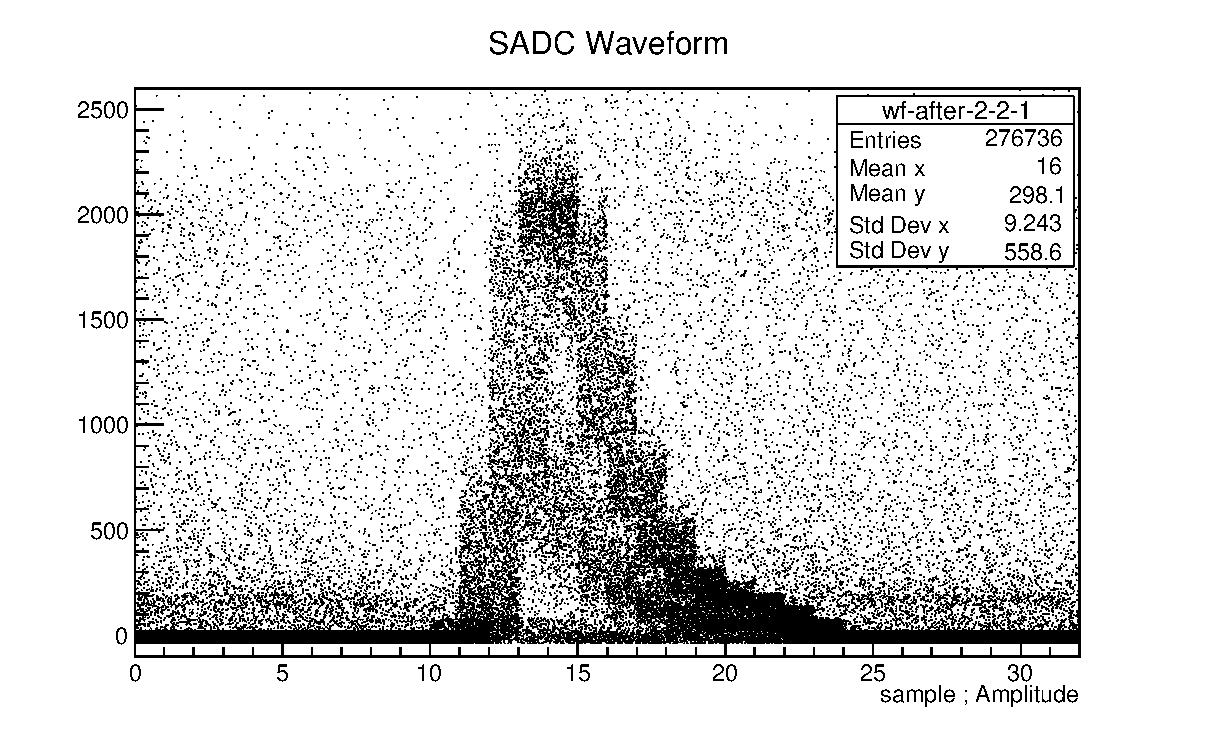
\includegraphics[width=0.65\linewidth]{images/illustrative/msadc-waveforms-example.eps}
    \caption{Гистограмма характеризующая временную развёртку амплитудного сигнала в
    центральной ячейке от моноэнергетического пучка}
    \label{fig:msadc-example}
\end{figure}

Для регистрации сигнала от сцинтилляционных детекторов в эксперименте
применяются ФЭУ-84~\cite{soviet_pmts}, для которых время нарастания
импульса анодного тока не превышает одной наносекунды. При этом
характерная длительность (ширина на половине амплитуды) импульсов от
большинства детекторов лежит в диапазоне от двух до трёх наносекунд.

Следует отметить, что согласно теореме Котельникова (Найквиста-Шеннона),
для безошибочного восстановления сигнала с таким характерным временем,
необходима частота дискретизации не менее $800\text{МГц}$ (частота
Найквиста для сигналов длительностью $2{,}4\text{нс}$).

С целью разрешения единичных импульсов от ФЭУ-84 в основном применяемых в
эксперименте, сигнал от \acrshort{pmt} передаётся сначала на вход
предварительного преобразователя (шейпера выполненого на основе
операционного усилителя AD8021~\cite{ad8021}), увеличивающего характерную
ширину сигнала примерно в три раза с сохранением амплитудной
пропорциональности. Несмотря
на то что частоты $80\text{МГц}$ всё ещё недостаточно для безошибочного
разрешения сигналов с полушириной в диапазоне от $6$ до $9~\text{нс}$
(частота Найквиста составляет примерно $170\text{МГц}$), необходимой
точности восстановления временных характеристик сигналов можно
добиться используя априорную информацию о форме сигнала -- то есть,
подобрав аналитическую модель достаточно хорошо воспроизводящую сигнал,
способную восполнить недостающую информацию в частотном домене.

\subsection{Параметризация сигнала АЦП}

С целью определения основных свойств сигнала и выбора оптимальных моделей для
математической подгонки (фита), для различных детекторов была выполнена серия
измерений формы импульса до и после шейпера с применением цифрового
осциллографа с пикосекундным разрешением.

%При рассмотрении малых амплитуд (менее $100~\text{мВ}$) определённую
%практическую трудность создают различные помехи, обусловленные индуктивными
%эффектами при работе на высоких частотах, такие как эффекты индуктивных
%задержек и отражений в коаксиальных проводниках, неидельность волнового
%сопротивления во цепи между шейпером и осциллографом или \acrshort{pmt} или
%осциллографом. С целью снижения этих эффектов при проверке модели
%параметризации, для проверки модели параметризации в области малых
%амплитуд, было выполнено численное моделирование шейпера на основе его
%принципиальной схемы.
Анализ сигналов малой амплитуды (менее $100~\text{мВ}$) имеет
определённые практические трудности, обусловленные влиянием помех,
связанных с индуктивными эффектами, проявляющимися при работе на высоких
частотах. К числу таких эффектов относятся индуктивные задержки и
отражения в коаксиальных линиях передачи, а также отклонения
волнового сопротивления от номинального в линии связи между
шейпером и осциллографом и между шейпером и \acrshort{pmt}.

Для уменьшения влияния указанных факторов при проверке работоспособности
модели параметризации в области малых амплитуд было выполнено численное
моделирование работы шейпера на основе его принципиальной электрической
схемы в программном пакете LTspice~\cite{ltspice}.

%На рисунке~\ref{fig:ltspice-shaper-simulation} показан пример временной
%развёртки сигнала. Импульсам с отрицательной амплитудой соответствуют
%запись входного сигнала выполненного осциллографом с интервалом
%200 пикосекунд. Импульс с положительной амплитудой отображает результат
%симуляции.

На рисунке~\ref{fig:ltspice-shaper-simulation} приведён пример временной
развёртки сигнала. Импульсы с отрицательной амплитудой соответствуют
результатам регистрации входного сигнала осциллографом с временным шагом
дискретизации 2~пс, тогда как импульс с положительной амплитудой
представляет собой результат компьютерного моделирования.

\begin{figure}
    \centering
    \includegraphics[width=0.75\linewidth]{images//illustrative/shaper-simulation.png}
    \caption{Результат моделирования преобразования сигнала в LTspice}
    \label{fig:ltspice-shaper-simulation}
\end{figure}

Моделирование достаточно хорошо (в пределах 1\%) согласуется с измеренным
выходным сигналом с амплитудами не менее нескольких десятков мВ.
На основании записанного сигнала в области больших
амплитуд, и с использованием численной модели LTspice, производилась проверка многопараметрических аналитических функций, способных воспроизводить форму
сигнала до или после шейпера.

%Количественные критерий, в виду сложной зависимости функции отклика от
%парамтров измерения, были сформулированы на основе важнейших физических
%параметров, а не общего численного соответствия. В частности, не
%рассматривалась точность поведения экспоненциального спадания импульса
%на интервалах превышающих ширину на полувысоте более чем вдвое, поскольку,
%в силу схемотехнических причин, последняя на этом участке слишком сильно
%зависит от парамтров шейпера имеющих большой разброс. Напротив, важными
%параметрами являлись:
Количественные критерии, учитывая сложную зависимость функции отклика
от параметров измерений, были определены на основе ключевых физических
характеристик, и в меньшей степени -- на основе общего численного
совпадения формы сигнала.
При этом не рассматривалась точность аппроксимации экспоненциального
спада импульса на временных интервалах, превышающих удвоенную ширину
на полувысоте, поскольку в данной области форма импульса существенно
зависит от параметров шейпера, характеризующихся значительным
технологическим разбросом.

В качестве основных критериев были выбраны:
\begin{itemize}
    \item Точка на переднем фронте импульса, соответствующая полувысоте
    импульса, принятая в качестве инвариантной временной метки (постоянная
    доля, англ. \emph{constant fraction}),
    \item Амплитуда в абсолютном максимуме импульса, как величина
    пропорциональная энерговыделению.
\end{itemize}

Помимо количественного соответствия сигналам, функции должны достаточно
просты для численного счёта, чтобы их можно было применять в различных
схемах нелинейной минимизации, таких как метод Ньютона, метод градиентного спуска
или алгоритм Левенберга-Марквардта~\cite{marquardt-lms}.

Итак, согласно выбранным критериям, рассматриваются следующие функции:

\begin{itemize}
    \item Функция Мояла \cite{moyalFunction} с тремя параметрами, определяемая выражением
    \begin{equation}
        F_M(t) = \frac{A}{\sqrt{2 \pi}} \exp \left\{ - \frac{1}{2} \left(\frac{x - \mu}{\sigma}+ \exp\left(\frac{x - \mu}{\sigma}\right)\right) \right\}
        \label{eq:moyalFNormed}
    \end{equation}
    которая адекватно описывает результат преобразования сигнала
    шейпером, позволяя использовать сравнительно простые аналитические формулы
    для временных характеристик (например, точки перегиба на переднем фронте) и амплитуды. Несмотря на присутствие быстро растущего множителя
    $e^{e^x}$, функция демонстрирует численную устойчивость при минимизации методом Левенберга–Марквардта с ускорением сходимости градиентом.
    \item Функция специального вида (N-pole), появляющаяся при различных
    аппроксимациях в некоторых статистических приложениях гамма-функции~\cite{gamma-stegun}:
    \begin{equation}
        f_{Np}\left(x\right)=A\left(x-t_{0}\right)^{n}e^{-\frac{\left(x-t_{0}\right)}{T}}\ \left\{x>t_{0}\right\}
    \end{equation}
    %хорошо описывает форму импульса до шейпера, воспроизводя быстрый рост
    %переднего фронта и обеспечивая устойчивые оценки
    %временных характеристик. При этом, аналитические выражения для времени
    %и амплитуды сигнала требуют вычисления специальных функций (гамма функции
    %и $W$ Ламберта). Из-за быстрого роста параметра $n$ функция требует
    %применения масштабных преобразований, иначе её сходимость нестабильна.
    %Также, при разрешении вкладов от близких по времени импульсов, функция
    %требует введения апостериорных ограничений для разрегения неоднозначности.
    которая хорошо воспроизводит форму импульса до шейпера, обеспечивая
    быстрое нарастание переднего фронта и стабильные оценки временных
    параметров. При этом аналитические выражения для времени и амплитуды
    сигнала требуют вычисления специальных функций --- гамма-функции и
    $W$-функции Ламберта. Из-за быстрого роста параметра $n$ функция
    требует применения масштабных преобразований для обеспечения
    сходимости численных алгоритмов. Кроме того, при разрешении
    наложенных импульсов с близкими по времени появлениями требуется
    введение апостериорных ограничений с целью устранения
    неоднозначностей.
    \item Четырёхпараметрическая функция из работы \cite{optimal-pulse-proc-samoyl}:
    \begin{equation}
        F(t) = A \cdot \exp(-(t-t_0)/\tau_1) /(1 + \exp(-(t-t_0)/\tau_2).
    \end{equation}
    %используется для аппроксимации импульсов с малой амплитудой. Практически,
    %независимость левого и правого фронтов приводят к необходимости
    %введения ограничений на основе апостериорных оценок.
    позволяющая независимо описывать участки нарастания и спада
    импульса. Эта функция применяется для аппроксимации сигналов
    малой амплитуды. Практически независимость параметров левого и
    правого фронтов требует введения апостериорных ограничений для
    обеспечения устойчивости.
\end{itemize}

%Применение описанных моделей позволяет описывать сигналы \acrshort{pmt}
%сэмплирующих АЦП в широком диапазоне энергий. В силу
%нелиности процедуры минимизации, наличия локальных
%минимумов, аппаратных шумов, а так же неоднозначности при разрешении
%вкладов от нескольких близких по времени частиц, практическое
%использование описанных параметризаций должно производиться в рамках
%программного окружения допускающего конкурентные сценарии,
%резервные алгоритмы условные ветвления и итеративную проверку гипотез.
Применение рассмотренных моделей позволяет адекватно описывать сигналы
\acrshort{pmt}, считываемые сэмплирующими АЦП в широком диапазоне энергий.
Ввиду нелинейности процедуры минимизации, наличия локальных минимумов
функции ошибки, а также влияния аппаратных шумов и неоднозначности при
разложении сигналов, формируемых несколькими близкорасположенными
во времени частицами, практическое использование данных параметризаций
должно осуществляться в программном обеспечении, обеспечивающем
поддержку конкурентных сценариев, резервных алгоритмов, условных
ветвлений и итеративной проверки гипотез.

\subsection{Уровень нулевого сигнала и эффекты высокой частоты}

%Уровнем нулевого сигнала (\emph{baseline}) называется значение оцифрованной
%амплитуды соответствующее отсутствию физического сигнала. Это значение
%обусловлено входным напряжением операционного усилителя во входном каскаде АЦП и
%балансировкой внутренних компараторов. Также, это значение определяется
%внутренними параметрами цепи и может быть подвержено
%незначительному дрейфу~($<1\%$), обусловленному изменениями гальванических
%характеристик линий преобразователя или изменением темнового тока \acrshort{pmt}
%под воздействием высокой интенсивности, термическими
%эффектами схемы, статистическими флуктуациями электронной лавины.
\emph{Уровнем нулевого сигнала} (\emph{baseline}) представляет собой значение оцифрованной амплитуды, соответствующее отсутствию сигнала на входе АЦП.
Формирование данного уровня обусловлено входным напряжением операционного
усилителя, используемого во входном каскаде АЦП, а также балансировкой
внутренних компараторов. Помимо этого, значение нулевого уровня определяется
внутренними параметрами входной цепи и может подвергаться незначительному
дрейфу (порядка $1 \%$ от уровня сигнала, что способно оказать заметное
влияние на разрешение некоторых детекторов), вызванному изменением
гальванических характеристик линий преобразователя, вариациями темнового
тока \acrshort{pmt} под воздействием высокой интенсивности, термическими эффектами
в электронной схеме, а также статистическими флуктуациями электронной
лавины.

Для повышения точности реконструкции энерговыделения в калориметре
необходимо применять устойчивый алгоритм выделения нулевого уровня, который бы
в наименьшей мере подвержен влиянию дрейфа и эффектам связанным с
интенсивностью пучка.

Существующий алгоритм динамического вычисления нулевого уровня заключается
в анализе первых нескольких сэмплов амплитудного сигнала и опирается на
предположение о том что в них отсутствует фактический сигнал. Последнее
обстоятельство гарантируется триггерной системой в смысле сигналов от
первичных частиц отслеживаемых триггерными счётчиками. Практически, нередки
события, когда сигнал в детекторе присутствует и обусловлен гало пучка, 
вторичными частицами и т.д. Если разброс
минимального и максимального значений превышает некоторый заданный порог,
за уровень нулевого сигнала берётся минимальное значение, в противном случае,
вычисляются средние. Результат работы такого алгоритма определяется
абсолютным порогом. На рисунке~\ref{fig:baselineresults} слева изображён
вариант работы такого алгоритма в случае, когда в окне оцифровки присутствует
остаточный сигнал от предыдущего события с амплитудой не превышающий
порог. Для наглядности, справа приведён результат работы улучшенного
алгоритма предложенного автором на основе минимизации невязок вторых
производных (\emph{деинтерлейсинг}), вместе с изображением результатов
аппроксимации модельными функциями.

\begin{figure}
    \centering
    \includegraphics[width=0.33\linewidth]{images//illustrative/baselines-distorted.png}
    \includegraphics[width=0.33\linewidth]{images//illustrative/baselines-corrected.png}
    \caption{Отыскание нулевого уровня сигнала
    по первым сэмплам (слева) и на основе минимизации производных (справа)
    в относительных единицах}
    \label{fig:baselineresults}
\end{figure}

%В качестве иллюстрации, рассмотрим сигналы изображённые на рисунке ...

Появление отдельных событий на триггере установки определяется средней
интенсивностью пучка, и их число в любой конечный интервал времени является
случайной величиной, распределение которой соответствует закону
Пуассона~\cite{exp-methods-Abramov1977}.
Управляемая средняя частота триггерных событий
обычно выбирается таким образом чтобы влияние событий оказавшихся в пределах
одного временного окна считывания данных было не слишком велико (обычно
от 5 до 40\% в окне $400~\text{нс}$).

Идентификация таких событий имеет важное значение в первую очередь на этапе
калибровки, поскольку будет обуславливать систематическую ошибку средних
величин для заранее неизвестного энергетического вклада.

\iffalse
Руководствуясь первыми принципами возможно оценить статистический вклад от
таких событий с тем чтобы рассчитать соответствующие поправки, если известна
функция отклика от незашумлённых данных.

%Рассмотрим например детекторы, считывание данных с которых производится чипом
%MSADC (сэмплирующий АЦП) --- чип оцифровывает гальванический сигнал (обычно
%амплитудный испульс с \acrshort{pmt} после шейпера) в виде набора отдельных измерений с
%фиксированным интервалоом в пределах короткого временного окна. В качестве
%модельного приближения выберем далее функцию Мояла \cite{moyalFunction}:

%в которой, помимо положения максимума $\mu$ введём дополнительные параметры
%отвечающие за ширину и площадь ($\sigma$ и $S$):
%\begin{equation}
%    M(t, \vec{p}) = \frac{S}{\sqrt{2 \pi} \sigma} \exp\left\{ - \frac{1}{2} \left(\frac{t-\mu}{\sigma} + \exp\left(-\frac{t-\mu}{\sigma}\right)\right) \right\}.
%\label{eq:moyalF}
%\end{equation}

%Функцию \eqref{eq:moyalFNormed} обычно используют в качестве аналитической
%аппроксимации функции плотности распределения Ландау \cite{BockHEPFormulae}.

Задержка сигнальной линии относительно триггера выбирается таким
образом, чтобы разместить максимум импульса в середине сэмплирующего окна,
а для вычисления пьедесталов производится по первым нескольким каналам таким
образом, чтобы им соответствовал вероятный ноль сигнала.

\begin{figure}[h]
    \centering
    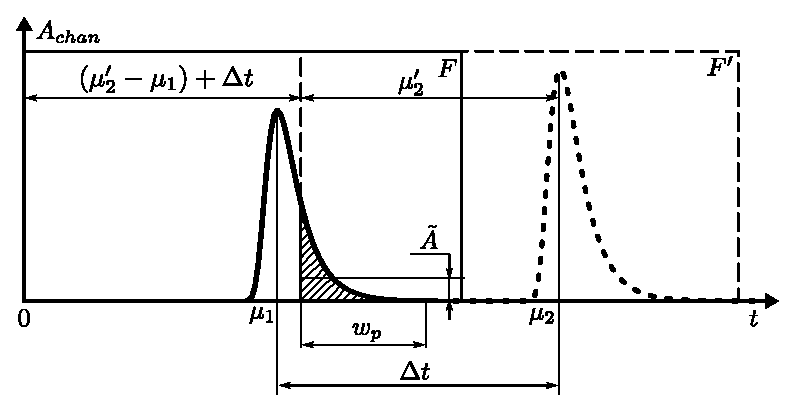
\includegraphics[scale=1.05]{pile-up-image-v2.eps}
    \caption{Схематическое изображение эффекта pile-up в амплитудно-временной
развёртке \acrshort{pmt}. Здесь, при оцифровке триггерного события (показано
пунктиром, вместе со своим окном дискретизации~$F'$) с максимальной
амплитудой в момент времени~$\mu_2 = \Delta t + \mu_2'$, в качестве значения
пьедестала будет взято среднее значение~$\tilde{A}$ на участке~$w_p$ которое
оказывается смещено относительно настоящего нуля за счёт вклада от события
$\mu_{1}$ (показано непрерывной линией вместе со своим окном дискретизации~$F$).}
    \label{fig:pileUpDiagram}
\end{figure}

Значение пьедестала $\tilde{A}$ определённое в окне
$w_p$, для каких-нибудь двух событий отклики которых заданы двумя наборами
параметров
$\mu_1, \sigma_1, S_1$ и $\mu_2, \sigma_2, S_2$, и произошедших с интервалом
$\Delta t$ можно записать в виде математического усреднения (см.
рис. \ref{fig:pileUpDiagram}):

\begin{equation}
\tilde{A} = \frac{1}{w_p} \int\limits_{\Delta t}^{\Delta t + w_p} (M(t, \mu_1, \sigma_1, S_1) + M(t, \mu_2, \sigma_2, S_2) \dd t
\end{equation}

Вклад $M(t, \mu_2, \sigma_2, S_2)$ будет ничтожным поскольку $w_p$ выбирается таким
образом, чтобы перекрыть участок до переднего фронта импульса триггерного
события, а дисперсия $\mu$ незначительна относительно ширины окна дискретизации
и $w_p$. Таким образом, модель можно редуцировать до плавающего окна усреднения
единственной функции $M(t, \mu_1, \sigma_1, S_1)$. Опустим индексы
для краткости, поскольку параметры триггерного события не влияют на результат: 

\begin{equation}
    \tilde{A}(\Delta t, \mu, \sigma, S) = \frac{1}{w_p} \int\limits_{0}^{w_p} M(t, \mu - \Delta t, \sigma, S) \dd t.
    \label{eq:avPedestal}
\end{equation}

Практический интерес представляет зависимость средней ошибки пьедестала от
средней частоты событий --- решение такой задачи даёт критерий для контроля
качества данных. Для того чтобы получить такую оценку аналитически, можно,
далее, взвесить и усреднить
функционал \eqref{eq:avPedestal} по $\Delta t$ и набору параметров
$\mu, \sigma, S$.


При этом, для правдоподобия модели критическое значение имеет
скоррелированность параметров $p_{n,(1)}$, --- в таком распределении
заключена основная информация о характере функции отклика единичного события.
Общий вид трёхмерной гистограммы распределения этих параметров показан на
рис. ???.
%TODO: 3D-гистограмма

Если каким-нибудь образом гарантировать отсутствие pile-up-событий в
гистограмме на рис. ???, то получившимся распределением можно воспользоваться
в качестве параметризации параметра модели.

Для частоты событий $\nu$ интервал между случайными событиями $\Delta t$
подчиняется экспоненциальному закону, таким образом среднее значение
пьедестала:

\begin{equation}
    \bar{A} (\nu) = \frac{\nu}{w_p} \int\limits_0^{\infty} \exp(- \Delta t \nu ) \left(
        \int\limits_{0}^{w_p} M(t, \mu - \Delta t, \sigma, S) \dd t \right) \dd \Delta t
\end{equation}
\fi
